\documentclass[aspectratio=1610]{beamer}
\usepackage[utf8]{inputenc}
\usepackage[T1]{fontenc}
\usepackage[german]{babel}
\usepackage[useregional]{datetime2}
\usepackage[nameinlink]{cleveref}
\usepackage[section]{placeins}
\usepackage{xcolor}
\usepackage{graphicx}
\usepackage{csquotes}
\usepackage{amsmath} % for $\text{}$
\usepackage{enumitem}
\usepackage{testbericht}
\usepackage{algorithm}
\usepackage{algorithmicx}
\usepackage{algpseudocode}
\usepackage{listings}
\usepackage{bera}
\usepackage{pdfpages}
\usepackage{colortbl}
\usepackage{chronosys}

\colorlet{punct}{red!60!black}
\definecolor{background}{HTML}{EEEEEE}
\definecolor{delim}{RGB}{20,105,176}
\colorlet{numb}{magenta!60!black}
\lstdefinelanguage{json}{
    basicstyle=\normalfont\ttfamily,
    numbers=left,
    numberstyle=\scriptsize,
    stepnumber=1,
    numbersep=8pt,
    showstringspaces=false,
    breaklines=true,
    frame=lines,
    backgroundcolor=\color{background},
    literate=
     *{0}{{{\color{numb}0}}}{1}
      {1}{{{\color{numb}1}}}{1}
      {2}{{{\color{numb}2}}}{1}
      {3}{{{\color{numb}3}}}{1}
      {4}{{{\color{numb}4}}}{1}
      {5}{{{\color{numb}5}}}{1}
      {6}{{{\color{numb}6}}}{1}
      {7}{{{\color{numb}7}}}{1}
      {8}{{{\color{numb}8}}}{1}
      {9}{{{\color{numb}9}}}{1}
      {:}{{{\color{punct}{:}}}}{1}
      {,}{{{\color{punct}{,}}}}{1}
      {\{}{{{\color{delim}{\{}}}}{1}
      {\}}{{{\color{delim}{\}}}}}{1}
      {[}{{{\color{delim}{[}}}}{1}
      {]}{{{\color{delim}{]}}}}{1},
}

\setlist{nosep}

\newcommand\urlpart[2]{$\underbrace{\text{\texttt{#1}}}{\text{#2}}$}
\raggedbottom
\crefname{figure}{Abb}{Abb}

\newcommand\producttitle{treff.}
\hypersetup{
	pdftitle={Testphase: \producttitle},
	bookmarks=true,
}

% header & footer
\usepackage{scrlayer-scrpage}
%\lofoot{\today}
%\refoot{\today}
\pagestyle{scrheadings}

\title{
\includegraphics[width = 50mm]{images/logo_crop.png}}
\subtitle{\huge Testphase}
\author{Lukas Dippon
	\and Jens Kienle
	\and Matthias Noll
    \\Fabian Röpke
	\and Tim Schmidt
	\and Simon Vögele}

\begin{document}

	\begin{frame}[plain]
	\maketitle
	\end{frame}

%%%%%%%% Vergleich mit Pflichtenheft %%%%%%%%%%

	\begin{frame}[plain]
        \frametitle{\textbf{Vergleich mit Pflichtenheft} -- Anforderungen}

        \begin{itemize}
          \item[-] einige Kür-Kriterien nicht oder teilweise erfüllt
          \item[-] keine Push-Benachrichtigungen \\
                   $\Rightarrow$ keine Chatbenachrichtigungen,
                   Standortanfragen etc
          \item[-] Nutzerkonten können nicht gelöscht werden \\
                   (schwerwiegende Lockingprobleme)
          \item[-] Material Design mehr als Richtlinien, weniger als Gesetz
          \item[-] Leistung bei hohem Nutzeraufkommen nicht garantiert
        \end{itemize}

  \end{frame}

  \begin{frame}[plain]
        \frametitle{\textbf{Vergleich mit Pflichtenheft} -- Testszenarien}

        \begin{itemize}
          \item[-] kleine Abweichungen in den Reaktionen \\
                   (Entwurfsänderung oder obige Probleme)
          \item[-] teilweise ungetestete Szenarien \\
                   (fehlende Implementierung)
          \item[-] Email wird nicht wie spezifiziert verwendet
        \end{itemize}

  \end{frame}

%%%%%%%% Server %%%%%%%%%%

	\begin{frame}[plain]
        \frametitle{\textbf{Server} -- Art der Tests und Überdeckung}
        82\% Zeilenabdeckung durch JUnit
        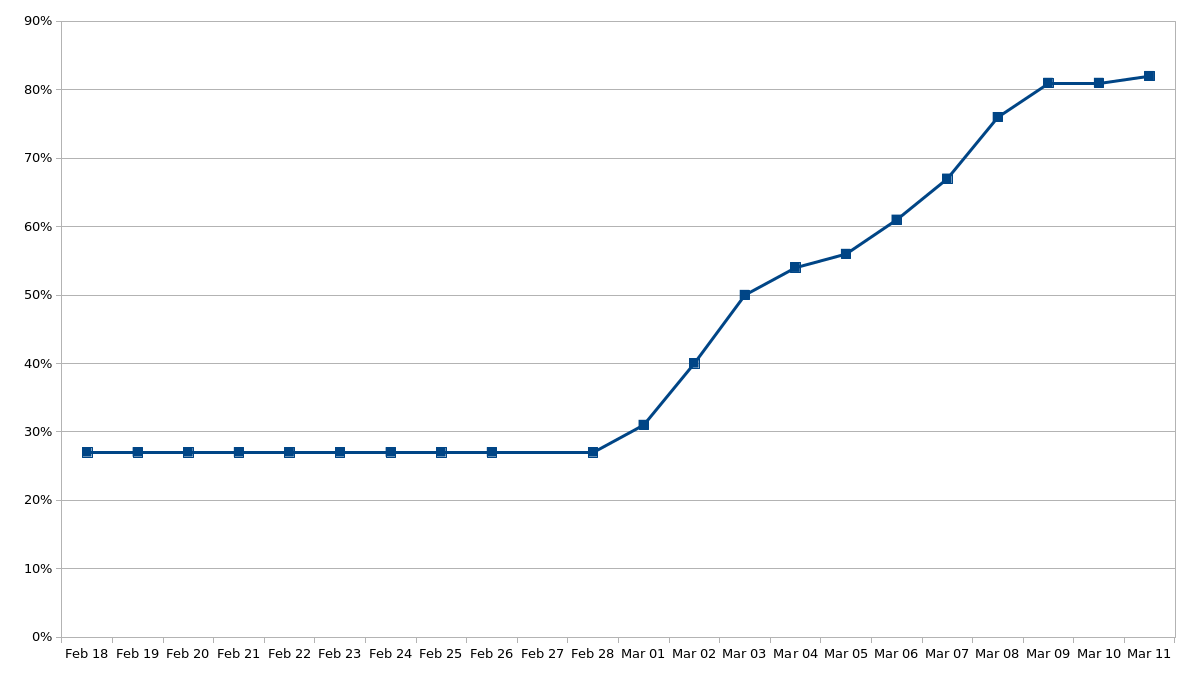
\includegraphics[width = \columnwidth * 9/10]{images/test-coverage-graph.png}
  \end{frame}

  \begin{frame}[plain]
        \frametitle{\textbf{Server} -- Art der Tests und Überdeckung}
        \begin{itemize}
            %TODO näher auf die Tests eingehen?
            \item[-] implementierte aber ungenutzte Befehle / Funktionen
            \item[-] Nebenläufigkeit getestet durch Szenarien
                  und Client-Debugging
        \end{itemize}
  \end{frame}

  \begin{frame}[plain]
        \frametitle{\textbf{Server} -- Probleme}

        \begin{itemize}
          \item[-] Nebenläufigkeit schwer testbar
          \item[-] Inkompetenz bei Verwendung des zur Verfügung
                   gestellten Servers
        \end{itemize}
  \end{frame}

  \begin{frame}[plain]
        \frametitle<1-3>{\textbf{Server} -- Deadlocks}
        \only<1>{
            \begin{figure}
                \begin{tabular}{ c | c | c }
                    \textbf{Test \#} & \textbf{Run \#} & \textbf{Result} \\
                    \hline
                    1 & 1 & \cellcolor{green!25}Works \\
                    1 & 2 & \cellcolor{green!25}Works \\
                    1 & 3 & \cellcolor{gray!25}Doesn't terminate \\
                    1 & 4 & \cellcolor{green!25}Works \\
                    1 & 5 & \cellcolor{gray!25}Doesn't terminate \\
                \end{tabular}
                \caption{Effektivität von Concurrency-Tests hängt vom Scheduler
                ab}
            \end{figure}
        }
        \only<2-3>{
            \begin{figure}
                \footnotesize
                \startchronology[startyear=1,stopyear=50,dates=false,
                arrowcolor=red,width=0.9\textwidth]
                \chronoevent{1}{\code{call execute()}}
                \chronoevent[markdepth=30pt]{13}{\code{readLock(x)}}
                \chronoevent{25}{\code{Set s = \{u,v,w,x,y,z\}}}
                \chronoevent[markdepth=30pt]{40}{\code{writeLockAllInSet(s)}}
                \chronoperiode[color=cyan]{13}{20}{CS 1}
                \chronoperiode[color=red,dates=false]{40}{50}{Deadlock}
                \stopchronology
                \caption{Deadlocks auch bei $\vert Threads\vert = 1$}
            \end{figure}
        }
        \only<3>{
            \centering{$\implies$ Statische Analyse nötig}
        }

    \end{frame}

%%%%%%%% Client %%%%%%%%%%

	\begin{frame}[plain]
        \frametitle{\textbf{Client} -- Titel}
    \end{frame}

%%%%%%%% Workflow %%%%%%%%%%

	\begin{frame}[plain]
        \frametitle{\textbf{Workflow} -- Titel}
    \end{frame}

%%%%%%%% Reflection %%%%%%%%%%

	\begin{frame}[plain]
        \frametitle{\textbf{Selbstreflexion} -- Titel}
    \end{frame}

\end{document}
